\documentclass[aspectratio=169,
				xcolor=table]{beamer}
\usepackage{ragged2e}
% Load general definitions
\usepackage[utf8]{inputenc}
%\usepackage[T1]{fontenc}
\usepackage[brazil]{babel}
\usepackage{amsmath}
\usepackage{amsfonts}
\usepackage{amssymb}
\usepackage{graphicx}
\usepackage{verbatim}
\usepackage{cancel}
\usepackage{askmaps}
\usepackage{tabularx}
\usepackage[table]{xcolor}
%\usepackage{tikz}
\usepackage{multirow}
\usepackage{mathtools}
\usepackage{color, colortbl}
\usepackage{etoolbox}
\usepackage{pbox}
\usepackage{changepage}
\usepackage{xpatch}
\usepackage{array}
\usepackage{marvosym}
\usepackage{tabu}
\usepackage{multicol}
\usepackage{listings}
\usepackage{underscore}
\usepackage{filecontents}
\usepackage[]{algorithm2e}
\usepackage{ragged2e}

\newcolumntype{P}[1]{>{\centering\arraybackslash}m{#1}}
\definecolor{Gray}{gray}{0.75}
\definecolor{Gray2}{gray}{0.85}

\definecolor{lightBlue}{HTML}{DAE8FC}
\definecolor{Blue}{RGB}{51, 51, 204}

%\useinnertheme[lily]{rounded}
\usetheme{UniEvangelica}
%\usetheme{Copenhagen}
%\usetheme{Berlin}
%\usecolortheme{dolphin}
\tolerance=1
\emergencystretch=\maxdimen
\hyphenpenalty=10000
\hbadness=10000

\setbeamertemplate{navigation symbols}{}%remove navigation symbols


\let\olditem=\item% 
\renewcommand{\item}{\olditem \justifying}%
\def\center{\trivlist \centering\item\relax}
\def\endcenter{\endtrivlist}

\setbeamertemplate{itemize/enumerate body begin}{\large}
\setbeamertemplate{itemize/enumerate subbody begin}{\large}

\setbeamertemplate{itemize item}{\raisebox{0.1ex}{$\blacktriangleright$}\hskip0.1em}
\setbeamertemplate{itemize subitem}{\raisebox{0.1ex}{$\blacktriangleright$}\hskip0.1em}

\newcommand{\greenarrow}{\textcolor{green}{\rotatebox[origin=c]{180}{\MVArrowDown}}}

\newcommand{\redarrow}{\textcolor{red}{\MVArrowDown}}

%\newcommand{\ftable}{
%	\begin{table}
%		\large
%		\centering
%		\rowcolors{1}{\ifnumless{\rownum}{2}{Blue}{lightBlue}}{}
%}

\newenvironment{eftable}{
	\begin{table}
		\large
		\centering
		\rowcolors{1}{}{Blue}
		\rowcolors{1}{\ifnumless{\rownum}{2}{Blue}{lightBlue}}{}
	}
	{
	\end{table}
}


%\setbeamertemplate{frametitle}
%{
%	%\vspace*{-2em}	
%	\insertframetitle
%
%	 %\textcolor{white}{\LARGE \insertframetitle}
%
%}

% Specific definitions
\institute[]{\uppercase{Engenharia de Software}}
\title[]{Unidade Central de Processamento}
\subtitle[]{\uppercase{Unidade Central de Processamento - CPU}}
\author[]{Prof. Alexandre Tannus}
\date{}

\AtBeginSection{\frame{\tableofcontents[currentsection]}}

\begin{document}

	\begin{frame}
		\titlepage
	\end{frame}
	\begin{frame}{Objetivos}
		\begin{itemize}
			\item Detalhar o funcionamento da Unidade Central de Processamento (CPU - \textit{Central Processing Unit})
			\vspace{0.35em}
			\item Entender a operação da Unidade Lógica Aritmética e como ela realiza cálculos básicos (soma e subtração)
			\vspace{0.35em}
			\item Compreender a função dos diversos registradores presentes na CPU
			\vspace{0.35em}
			\item Explicar as atribuições da unidade de controle
			\vspace{0.35em}
			\item Identificar os tipos de barramentos 
			\vspace{0.35em}
			\item Investigar o conjunto de instruções 
			\vspace{0.35em}
			\item Comparar os modelos de paralelismo que podem ser utilizados
		\end{itemize}
	\end{frame}

	\begin{frame}
		\tableofcontents		
	\end{frame}	
	
	\section{Introdução}
	\begin{frame}
		\frametitle{Unidade Central de Processamento (CPU)}
		\begin{itemize}
			\item \textit{Central Processing Unit} (CPU)
			\vspace{1em}
			\item Responsável pelos cálculos e controle da operação do computador

		\end{itemize}
		\begin{figure}
			\centering
			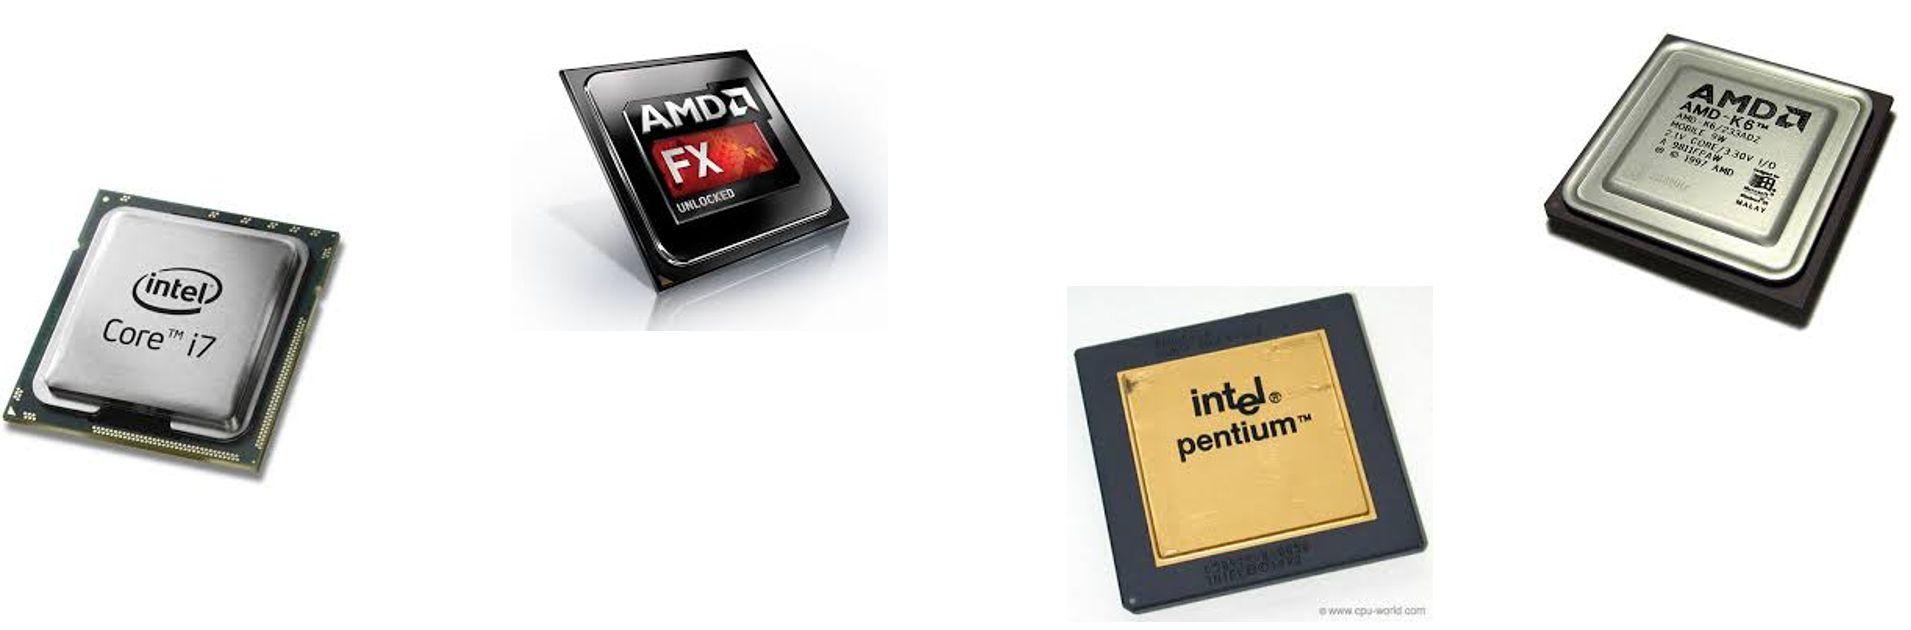
\includegraphics[height=3cm, keepaspectratio]{../figs/cap05/processadores.png} 
		\end{figure}
	\end{frame}
	
	\begin{frame}
		\frametitle{Estrutura da CPU}
		\begin{columns}
			\begin{column}{0.55\textwidth}
				\begin{itemize}
					\item Unidade lógica aritmética (ULA)
					\vspace{1em}
					\item Unidade de controle (UC)
					\vspace{1em}
					\item Registradores
					\vspace{1em}
					\item Barramentos

				\end{itemize}
			\end{column}
			\begin{column}{0.3\textwidth}
				\vspace{-0.5cm}
				\begin{figure}
					\centering
					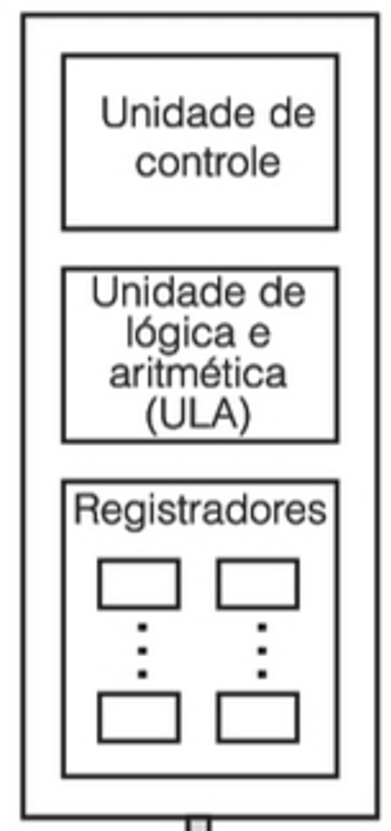
\includegraphics[height=5cm, keepaspectratio]{../figs/cap05/composicao.png} 
				\end{figure}				
			\end{column}
		\end{columns}
	\end{frame}
	
	\section{Unidade Lógica Aritmética}
		\begin{frame}
			\frametitle{CPU - Unidade Lógica Aritmética}
			\begin{itemize}
				\item Realiza as operações lógicas e aritméticas
				\begin{itemize}
					\item NOT, OR, AND
					\item Adição, Subtração
					\item Comparação
					\item Deslocamento
				\end{itemize}				
			\end{itemize}
			\begin{figure}
			\vspace{-1.5cm}
				\centering
				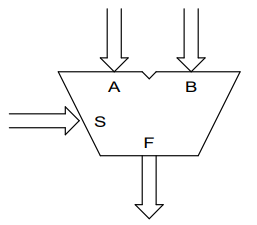
\includegraphics[height=0.6\textheight, keepaspectratio]{../figs/cap04/ula} 
			\end{figure}
		\end{frame}
		
		\begin{frame}
			\frametitle{Projeto da ULA - Representação de números}
				\begin{itemize}
					\item Inteiros sinalizados
					\begin{itemize}
						\item Sinal-magnitude
						\item \alert{Complemento de 2}
					\end{itemize}
					\vspace{1em}
					\item Ponto Flutuante
					\begin{itemize}
						\item \alert{Padrão ANSI/IEEE}
					\end{itemize}
				\end{itemize}
		\end{frame}		

		\begin{frame}
			\frametitle{Representação de inteiros: Sinal-magnitude}
			\begin{itemize}
				\item Bit mais significativo (MSB - \textit{Most Significant Bit}) indica o sinal
				\begin{itemize}
					\item 1: número negativo
					\item 0: número positivo
				\end{itemize}
			\end{itemize}
		\end{frame}		
	
		\begin{frame}
			\frametitle{Representação de inteiros: Complemento de 2}
			\begin{itemize}
				\item Representação de números negativos mais comum em hardware
	%			\pause
				\vspace{0.4em}
				\item Complemento de 1 $\to$ inversão bit a bit do número (complemento)
				\item Complemento de 2 $\to$ adição de 1 ao complemento de 1	
	%			\pause		
				\vspace{0.3em}
			\end{itemize}
			\begin{exampleblock}{Exemplos (representação em \textbf{8 bits})}
				\begin{columns}
					\begin{column}{0.45\textwidth}
						\begin{itemize}
							\item $9+4$
							\item $9-4$
						\end{itemize}
					\end{column}
					\begin{column}{0.45\textwidth}
						\begin{itemize}
							\item $-9+4$
							\item $-9-4$
						\end{itemize}
					\end{column}
				\end{columns}
			
			\end{exampleblock}
			
		\end{frame}		
		
		\begin{frame}
			\frametitle{Representação de ponto flutuante }
			\begin{eftable}
				\begin{tabular}{l | l | l}
					\textcolor{white}{Característica} &
					\textcolor{white}{Único/Curto} &
					\textcolor{white}{Duplo/Longo} \\
					Largura da palavra & 32 & 64 \\
					Bits mantissa & 23 & 52 \\
					Intervalo mantissa & $[1, 2-2^{-23}]$ & $[1, 2-2^{-52}]$\\
					Bits de expoente & 8 & 11 \\
					Excesso do expoente & 127 & 1023 \\
					Mínimo & $2^{-126} \approx 1,2x10^{-38}$ & $2^{-1022}\approx 2,2x10^{-308}$ \\
					Máximo & $2^{128} \approx 3,4x10^{-38}$ & $2^{1024}\approx 1,8x10^{308}$
				\end{tabular}
			
			\end{eftable}
		\end{frame}

		\begin{frame}
			\frametitle{Meio Somador - \textit{Half Adder}}
			\begin{columns}
				\begin{column}{0.3\textwidth}
					\begin{eftable}
						\begin{tabular}{c|c||c|c}		
							\textcolor{white}{x} & 
							\textcolor{white}{y} & 
							\textcolor{white}{s} & 
							\textcolor{white}{c} \\
							0 & 0 & 0 & 0 \\ 
							0 & 1 & 1 & 0 \\ 
							1 & 0 & 1 & 0 \\ 
							1 & 1 & 0 & 1 \\
						\end{tabular}		
					\end{eftable}				
				\end{column}
				\begin{column}{0.2\textwidth}
				\begin{figure}
					\hspace{-1cm}
					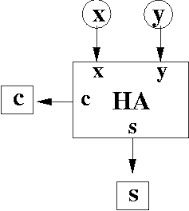
\includegraphics[height=3.4cm, keepaspectratio]{../figs/cap05/halfAdder.png} 
				\end{figure}
				\end{column}
				\begin{column}{0.5\textwidth}
					\begin{exampleblock}{Exemplos}
						\begin{itemize}
							\item $(11001)_2 + (1011)_2$ \\ 
		%					\pause
							\item $(101101)_2 + (11100111)_2$ \\ 
		%					\pause
							\item $(100111)_2 + (1110)_2 + (1011)_2 $			
						\end{itemize}
		
					\end{exampleblock}
				\end{column}
			\end{columns}
		\end{frame}

		\begin{frame}
			\frametitle{Somador Completo - \textit{Full Adder}}
			\begin{columns}
				\begin{column}{0.3\textwidth}
					\begin{eftable}
						\begin{tabular}{c|c|c||c|c}				
							\textcolor{white}{A} & 		
							\textcolor{white}{B} & 		
							\textcolor{white}{C-IN} & 		
							\textcolor{white}{C-OUT} & 		
							\textcolor{white}{SUM} \\ 
							0 & 0 & 0 & 0 & 0 \\ 
							0 & 0 & 1 & 0 & 1 \\ 
							0 & 1 & 0 & 0 & 1 \\ 
							0 & 1 & 1 & 1 & 0 \\ 
							1 & 0 & 0 & 0 & 1 \\ 
							1 & 0 & 1 & 1 & 0 \\ 
							1 & 1 & 0 & 1 & 0 \\ 
							1 & 1 & 1 & 1 & 1 \\ 
						\end{tabular} 
					\end{eftable}
				\end{column}
				\begin{column}{0.7\textwidth}
					\begin{figure}
						\centering
						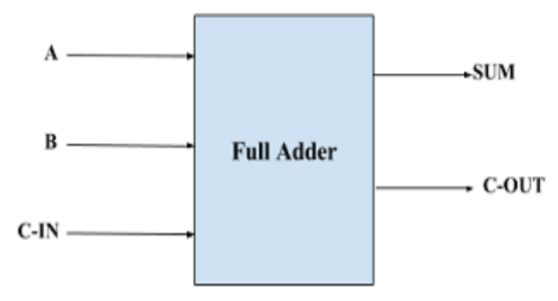
\includegraphics[width=.8\textwidth, keepaspectratio]{../figs/cap05/fullAdder.png} 
					\end{figure}
				\end{column}
			\end{columns}			
			
		\end{frame}

	\section{Registradores}
		\begin{frame}
			\frametitle{CPU - Registradores}
			\begin{itemize}
				\item Armazenam dados e instruções
				\vspace{1em}
				\item Baixa capacidade de armazenamento
				\vspace{1em}
				\item Alta velocidade de acesso
				\vspace{1em}
				\item Podem ser
				\begin{itemize}
					\item Propósito geral - operações lógicas e aritméticas
					\item Especiais - Acumuladores, \textit{Program Counter}, registrador de \textit{flags}, etc.
				\end{itemize}
				
			\end{itemize}
		\end{frame}
		
		\begin{frame}
			\frametitle{Registradores importantes}
			\begin{itemize}
				\item Contador de programa (\textit{Program Counter} - PC)	
				\begin{itemize}
					\item Armazena o endereço de memória onde será lida a próxima instrução que será executada
					\item Atualizado após a busca da instrução
				\end{itemize}
				\vspace{1em}
				\item Registrador de Instrução (\textit{Instruction Register} - IR)
				\begin{itemize}
					\item Armazena a instrução em execução
				\end{itemize}
			\end{itemize}
		\end{frame}
		
		\begin{frame}
			\frametitle{Registradores importantes}
			\begin{itemize}
			 \item Registrador de endereços de memória (\textit{Memory Address Registers} - MAR)
			 \vspace{1em}
			 \item Registrador \textit{buffer} de memória - (\textit{Memory Buffer Register} - MBR)
			\end{itemize}
			
			\vspace{1em}
			\Large \alert{Registradores responsáveis pela troca de informações (dados e instruções) entre memória e CPU}
		\end{frame}
		
		\begin{frame}
			\frametitle{Registradores importantes}
			\begin{itemize}
				\item Palavra de estado do programa ( \textit{Program State Word} - PSW)
				\vspace{1em}
				\item Informações de estado 
				\begin{itemize}
					\item sinal
					\item zero
					\item \textit{carry}: \textit{carry out} bit de uma operação
					\item \textit{overflow}
					\item  \textit{interrupt enable/disable}: habilita ou desabilita interrupções
				\end{itemize}
			\end{itemize}
		\end{frame}
		
		\begin{frame}
			\frametitle{Registradores de uso geral - Intel x86}
			\begin{itemize}
				\item AX - Acumuladores
				\item BX - Base
				\item CX - Contador
				\item DX - Dados
				\item BP - Ponteiro de base
				\item SI e DI - usado em operações que envolvem \textit{strings}
			\end{itemize}
			
		\end{frame}

	\section{Unidade de Controle}		
		\begin{frame}
			\frametitle{CPU - Unidade de Controle}
			\begin{itemize}
				\item Controla toda a operação do microprocessador
				\vspace{1em}
				\item Constituída por
				\begin{itemize}
					\item Circuito de temporização
					\item Controle e decodificação
					\item Decodificador de instruções
				\end{itemize}
			\end{itemize}
		\end{frame}

	\section{Barramentos}	
	
	\begin{frame}
		\frametitle{Barramentos}
		\begin{itemize}
			\item Vias que interligam os dispositivos (CPU, memória e periféricos), permitindo a comunicação entre os mesmos.
			\vspace{1em}
			\item Três tipos
			\begin{itemize}
				\item Dados
				\item Endereços
				\item Controle
			\end{itemize}
		\end{itemize}
		\begin{minipage}{\textwidth}
		
				\vspace*{-3cm}
			\begin{figure}
				\centering
				\hspace*{5cm}
				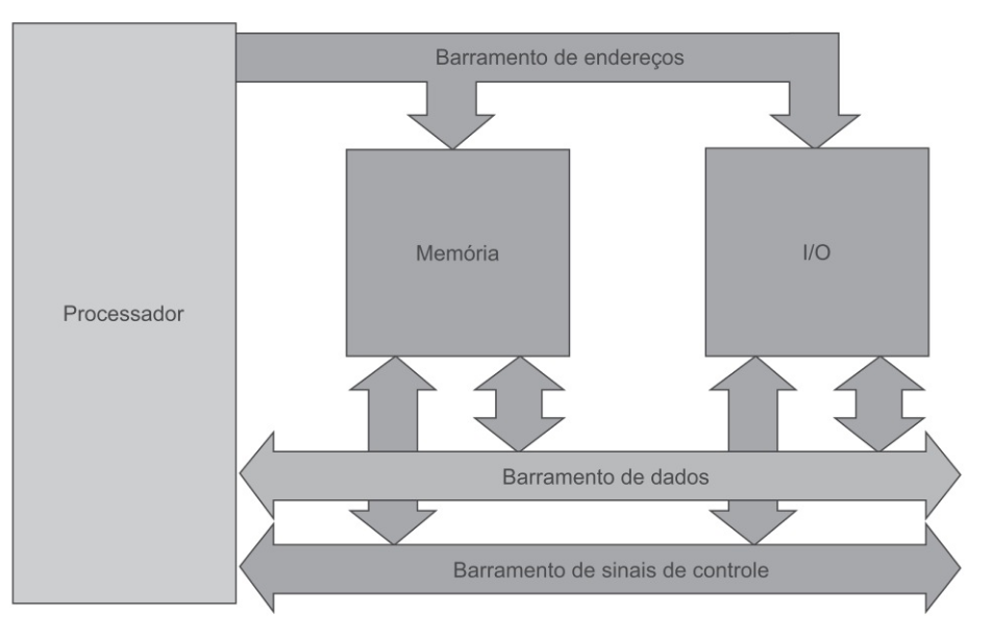
\includegraphics[width=.65\textwidth, keepaspectratio]{../figs/cap05/barramento.png}
			\end{figure}		
		\end{minipage}
	\end{frame}
	
	\begin{frame}
		\frametitle{Barramento de dados}
		
		\begin{itemize}
			\item Trafega dados, informações ou instruções 
			\vspace{1em}
			\item Composto por vias
			\begin{itemize}
				\item Cada via trafega um bit
				\item Quantidade de vias define largura do barramento

			\end{itemize}
			\vspace{1em}
			
			\item \alert{ATENÇÃO: Largura do barramento de dados pode ser diferente da quantidade de bits que o processador utiliza} 			

		\end{itemize}
	\end{frame}
	
	\begin{frame}
		\frametitle{Barramento externo \textit{vs.} processamento interno}
		\begin{eftable}
			\begin{tabular}{l | c | c}
				\textcolor{white}{Processador} &
				\textcolor{white}{Processamento interno} &
				\textcolor{white}{Barramento externo} \\
				i8080 (1974) & 8 & 8 \\
				8088 (1979) & 16 & 8 \\
				80286 (1982) & 8 & 16 \\
				80386DX (1985) & 32 & 32 \\
				80486DX (1989) & 32 & 32 \\
				Pentium (1993) & 32 & 64 \\
				Athlon 64 (2003) & 64 & 128 			
			\end{tabular}
		\end{eftable}
	\end{frame}
	
	\begin{frame}
		\frametitle{Barramento de endereços}
		\begin{itemize}
			\item Endereçamento dos periféricos do sistema
			\begin{itemize}
				\item Memórias
				\item Controlador de vídeo
				\item Disco
				\item Rede

			\end{itemize}
			\vspace{1em}
			\item Quantidade de vias define quantidade máxima de endereços possíveis

		\end{itemize}
	\end{frame}
	
	\begin{frame}
		\frametitle{Barramento de endereço}
		\begin{eftable}
			\begin{tabular}{l | m{0.3\textwidth} | m{0.25\textwidth}}
				\textcolor{white}{Processador} & 
				\textcolor{white}{Largura do barramento  de endereços} & 
				\textcolor{white}{Quantidade máxima de endereços} \\
				i8088       & 20 bits & 1 Mb \\
				i80286      & 24 bits & 16 Mb \\
				i386        & 32 bits & 4 Gb  \\
				Pentium     & 32 bits & 4 Gb \\
				Core i5     & 35 bits & 32 Gb                         
			\end{tabular}
		\end{eftable}
	\end{frame}
	
	\begin{frame}
		\frametitle{Barramento de controle}
		\begin{itemize}
			\item Recebimento/envio de sinais de controle para os dispositivos do sistema
			\begin{itemize}
				\item RESET
				\item Interrupções
				\item HALT
				\item HOLD
				\item Seleção

			\end{itemize}
			\vspace{1em}
			\item Sinais de controle são específicos de cada arquitetura
		\end{itemize}
	\end{frame}
	
		
	\section{Instruções}

	\begin{frame}
		\frametitle{Conjunto de Instruções}
		\begin{itemize}
			\item Interface entre o programador e a máquina
			\vspace{1em}
			\item Cada instrução realiza uma tarefa simples
			\vspace{1em}
			\item Operações complexas podem ser construídas a partir de operações simples
		\end{itemize}
	\end{frame}
	
%	\begin{frame}
%		\frametitle{Exemplo}
%		\begin{lstlisting}
%add		$t8, $s2, $s3
%add		$t9, $s5, $s6
%add		$s7, $t8, $t9
%		\end{lstlisting}
%	\end{frame}	
	
	\begin{frame}
		\frametitle{Formato das instruções}
		\begin{itemize}
			\item Execução sequencial
			\vspace{1em}
			\item Exceções
			\begin{itemize}
				\item Instruções de salto
				\item Instruções de desvio
			\end{itemize}
		\end{itemize}
	\end{frame}
	
	\begin{frame}
		\frametitle{Tipos de instruções}
		\begin{eftable}
		\Large
		\resizebox{\textwidth}{!}{
		\begin{tabular}{@{}  c | m{3cm} | m{2.5cm} | m{2.5cm} | m{2.5cm} | m{2.5cm} | m{3cm} @{}}
			
			\textcolor{white}{Tipo} &
			\multicolumn{6}{|c|}{\textcolor{white}{Formato (bits)}} \\
			
			R & opcode (6) & rs(5) & rt(5) & rd(5) & shamt(5) & function(6) \\
			
			I & opcode (6) & rs(5) & rt(5) & \multicolumn{3}{|c|}{imediato(16)} \\
			
			J & opcode(6) & \multicolumn{5}{|c|}{endereço(26)} \\
			
		\end{tabular}}
		\end{eftable}
	\end{frame}
	
	\begin{frame}
		\frametitle{Instruções Aritméticas e Lógicas Básicas}
		
		\begin{eftable}
			\begin{tabular}{c |c |l | c}
			 \textcolor{white}{Operação} & 
			 \textcolor{white}{Comando} & 
			 \textcolor{white}{Sintaxe} &
			 \textcolor{white}{Função} \\
			 Adição & $add$ & $add \quad \$t0, \$s0, \$s1$ & 32\\
			 Subtração & $sub$ & $sub \quad \$t0, \$s0, \$s1$ & 34\\
			 Lógica AND & $and$ & $and \quad \$t0, \$s0, \$s1$ & 36\\
			 Lógica OR & $or$ & $or \quad \$t0, \$s0, \$s1$ & 37\\
			 Lógica XOR & $xor$ & $xor \quad \$t0, \$s0, \$s1$ & 38\\
			 Lógica NOR & $nor$ & $nor \quad \$t0, \$s0, \$s1$ & 39\\

			 Adição imediata& $addi$ & $addi \quad \$t0, \$s0, constante$ & 8\\	
			 Lógica AND imediata& $andi$ & $andi \quad \$t0, \$s0, constante$ & 12\\
			 Lógica OR imediata& $ori$ & $ori \quad \$t0, \$s0, constante$ & 13\\
			 Lógica XOR imediata& $xori$ & $xori \quad \$t0, \$s0, constante$ & 14\\

			\end{tabular}
		\end{eftable}
	\end{frame}

	\begin{frame}
		\frametitle{Instruções de Carga e Armazenamento }
		\begin{itemize}
			\item Transferência de 32 bits entre memória e registradores
			\vspace{1em}
			\item Instrução tipo I
			\vspace{1em}
			\item Regsitrador \textit{rt} - destino (\textit{load}) ou origem (\textit{store)}
			\vspace{1em}
			\item Endereço de memória - Constante de deslocamento + valor do registrador \textit{rs}
		\end{itemize}
	\end{frame}
	
	\begin{frame}
		\frametitle{Instruções de Salto e Desvio}
		\begin{itemize}
			\item Alteram o fluxo de execução sequencial
			\vspace{1em}
			\item Salto
			\begin{itemize}
				\item Instrução \textit{j} ou \textit{jr}
			\end{itemize}
			\vspace{1em}
			\item Desvio
			\begin{itemize}
				\item \textit{bne} - diferente de
				\item \textit{bltz} - menor que
				\item \textit{beq} - igual a
			\end{itemize}
		\end{itemize}
	\end{frame}
	
	\begin{frame}
		\frametitle{Modos de endereçamento}
		\begin{itemize}
			\item Implícito
			\item Imediato
			\item Por registrador
			\item Base
			\item Relativo ao PC
			\item Pseudodireto
		\end{itemize}
	\end{frame}
	
	
	\begin{frame}
		\frametitle{Ciclo de Instrução}
		\begin{itemize}
			\item Busca
			\begin{itemize}
				\item Leitura da próxima instrução da memória
			\end{itemize}
			\vspace{1em}
			\item Execução
			\begin{itemize}
				\item Interpretação e efetuação da operação indicada
			\end{itemize}
			\vspace{1em}
			\item Interrupção
			\begin{itemize}
				\item Verificação de ocorrência de interrupção
			\end{itemize}
		\end{itemize}
	\end{frame}
	
	\begin{frame}
		\frametitle{Ciclo de instrução}
		\begin{figure}
			\centering
			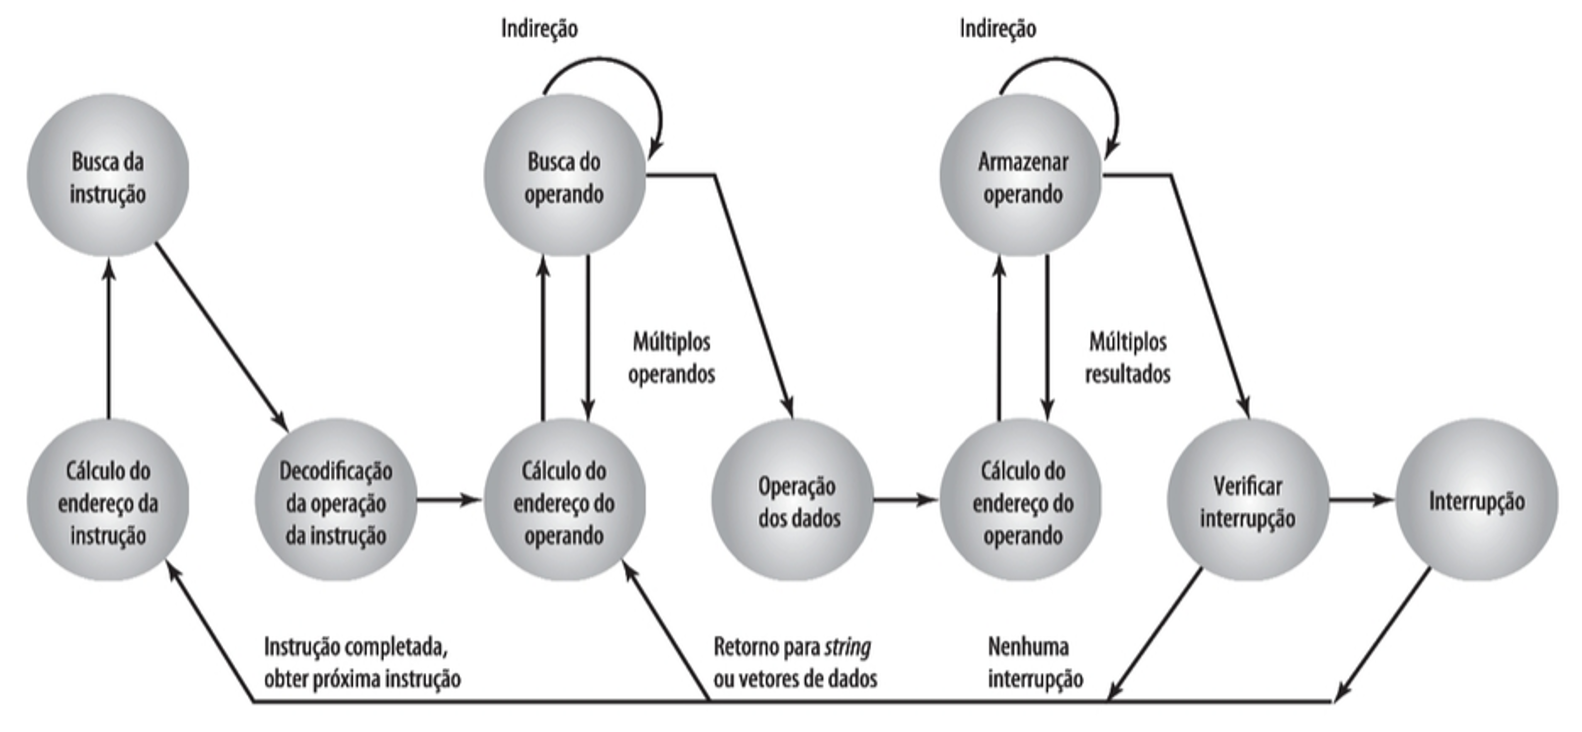
\includegraphics[height=0.8\textheight , keepaspectratio]{../figs/cap05/intrucao.png} 
		\end{figure}
	\end{frame}
	
	\begin{frame}
		\frametitle{Arquitetura CISC}
		\begin{itemize}
			\item Anos 80 – computadores mais complexos
			\vspace{1em}

			\item CISC – \textit{Complex Instruction Set Computer}
			\vspace{1em}

			\item Conjuntos de instruções cada vez mais complexas e maiores
			\begin{itemize}
				\item Pode afetar o desempenho
				\item Maior dificuldade de implementação de outras funções

			\end{itemize}

		\end{itemize}
	\end{frame}
	
	\begin{frame}
		\frametitle{Arquitetura RISC}
		\begin{itemize}
			\item RISC – \textit{Reduced Instruction Set Computer}
			\vspace{1em}

			\item Diminuição do número de instruções disponíveis
			\vspace{1em}
			
			\item Padronização do tamanho das instruções
			\vspace{1em}

			\item Introdução do pipeline
		\end{itemize}
	\end{frame}
	
	\begin{frame}
		\frametitle{Arquitetura RISC}
		\begin{itemize}
			\item Controle via \textit{hardware}
			\vspace{1em}
			\item Maior número de registradores
			\vspace{1em}
			\item Modos de endereçamento limitados
		\end{itemize}
	\end{frame}
	
	\section{Paralelismo}	
	
	\begin{frame}
		\frametitle{Paralelismo}
		\begin{itemize}
			\item Realizar várias coisas ao mesmo tempo
			\vspace{1em}	
			\item Dois níveis
			\begin{itemize}
				\item Instrução
				\item Processador
			\end{itemize}

		\end{itemize}
	\end{frame}
	
	\begin{frame}
		\frametitle{Paralelismo de instrução}
		\begin{itemize}
			\item Executar mais instruções em um determinado tempo
			\vspace{1em}
			\item Dois modelos
			\begin{itemize}
				\item \textit{Pipelines}
				\item Superescalares
			\end{itemize}

		\end{itemize}
	\end{frame}
	
	\begin{frame}
		\frametitle{\textit{Pipeline}}
		\begin{itemize}
			\item Dividir uma instrução em vários estágios

			\item Dedicar uma parte do \textit{hardware} para cada estágio

			\item Executar paralelamente vários estágios 

		\end{itemize}
	\end{frame}

	\begin{frame}
		\frametitle{\textit{Pipeline} de 6 estágios}
		\begin{figure}
			\centering
			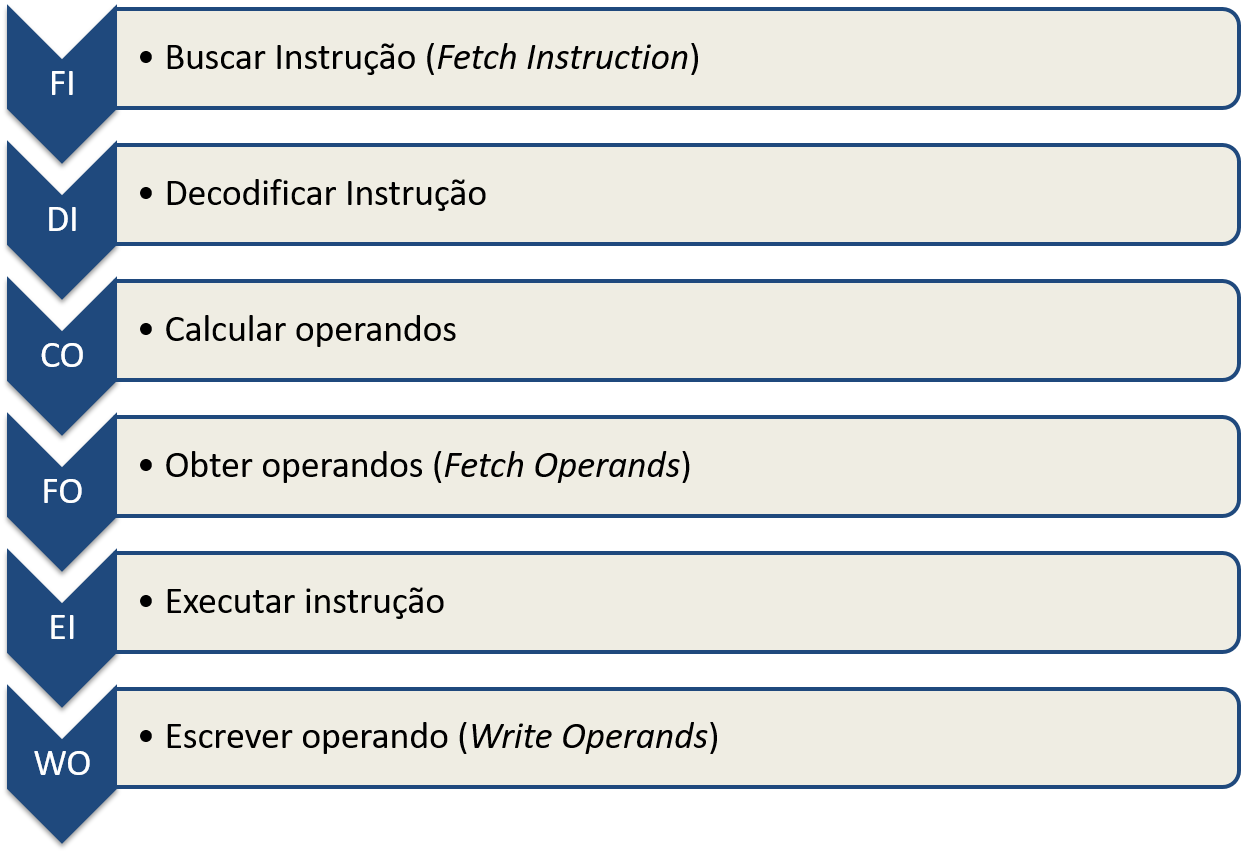
\includegraphics[height=0.8\textheight , keepaspectratio]{../figs/cap05/pipeline01.png} 
		\end{figure}
	\end{frame}
	
	\begin{frame}[t]
		\frametitle{\textit{Pipeline} de 6 estágios}
		\begin{itemize}
			\item Buscar Instrução (Fetch Instruction)
			\begin{itemize}
				\item Leitura da próxima instrução 
			\end{itemize}
			\vspace{1em}
			\item Decodificar Instrução
			\vspace{1em}
			\item Calcular operandos
			\begin{itemize}
				\item Cálculo do endereço efetivo de cada operando
			\end{itemize}

		\end{itemize}
	\end{frame}

	\begin{frame}
		\frametitle{\textit{Pipeline} de 6 estágios}
		\begin{itemize}
			\item Obter operandos (Fetch Operands)
			\begin{itemize}
				\item Obtenção dos operandos da memória
			\end{itemize}
			\vspace{1em}
			\item Executar Instrução
			\begin{itemize}
				\item Realização da operação e armazenamento do resultado no registrador
			\end{itemize}
			\vspace{1em}
			\item Escrever operandos (\textit{Write Operands})
			\begin{itemize}
				\item Cálculo do endereço efetivo de cada operando
			\end{itemize}

		\end{itemize}
	\end{frame}
	
	\begin{frame}[t]
		\frametitle{Executando instruções}

		\begin{eftable}
		\resizebox{\textwidth}{!}{
			\begin{tabular}{@{} l *{18}{c} @{}}
	            & 
	            \textcolor{white}{1}  & \textcolor{white}{2}  & 
	            \textcolor{white}{3}  & \textcolor{white}{4}  & 
	            \textcolor{white}{5}  & \textcolor{white}{6}  & 
	            \textcolor{white}{7}  & \textcolor{white}{8}  & 
	            \textcolor{white}{9}  & \textcolor{white}{10} & 
	            \textcolor{white}{11} & \textcolor{white}{12} & 
	            \textcolor{white}{13} & \textcolor{white}{14} & 
	            \textcolor{white}{15} & \textcolor{white}{16} & 
	            \textcolor{white}{17} & \textcolor{white}{18} \\
				Instrução 1 & FI & BI & CO & FO & EI & W0 &    &    &    &    &    &    &    &    &    &    &    &    \\
				Instrução 2 &    &    &    &    &    &    & FI & BI & CO & FO & EI & WO &    &    &    &    &    &    \\
				Instrução 3 &    &    &    &    &    &    &    &    &    &    &    &    & FI & BI & CO & FO & EI & WO
			\end{tabular}}
		\end{eftable}
	\end{frame}

	\begin{frame}
		\frametitle{Executando instruções}

		\begin{eftable}
		\resizebox{\textwidth}{!}{
			\begin{tabular}{@{} l *{18}{c} @{}}
	            & 
	            \textcolor{white}{1}  & \textcolor{white}{2}  & 
	            \textcolor{white}{3}  & \textcolor{white}{4}  & 
	            \textcolor{white}{5}  & \textcolor{white}{6}  & 
	            \textcolor{white}{7}  & \textcolor{white}{8}  & 
	            \textcolor{white}{9}  & \textcolor{white}{10} & 
	            \textcolor{white}{11} & \textcolor{white}{12} & 
	            \textcolor{white}{13} & \textcolor{white}{14} & 
	            \textcolor{white}{15} & \textcolor{white}{16} & 
	            \textcolor{white}{17} & \textcolor{white}{18} \\
								
				Instrução 1 & FI & BI & CO & FO & EI & W0 &    &    &   &    &    &    &    &    &    &    &    &    \\
				Instrução 2 &    & FI & BI & CO & FO & EI & WO &    &   &    &    &    &    &    &    &    &    &    \\
				Instrução 3 &    &    & FI & BI & CO & FO & EI & WO &   &    &    &    &    &    &    &    &    &   
			\end{tabular}}
		\end{eftable}
	\end{frame}
	
	\begin{frame}
		\frametitle{Superescalares}
		\begin{itemize}
			\item Execução de vários \textit{pipelines} simultaneamente

		\end{itemize}
		\begin{figure}
			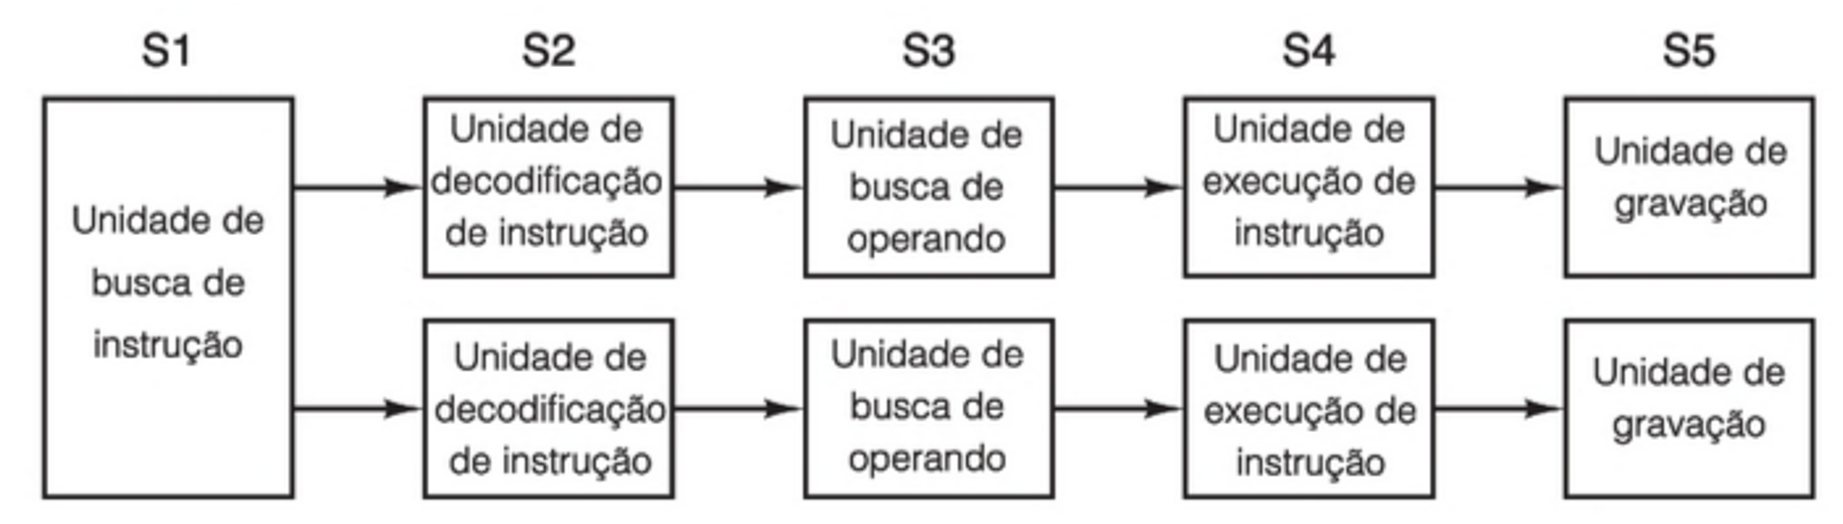
\includegraphics[width=\textwidth , keepaspectratio]{../figs/cap05/pipeline02.png} 
		\end{figure}
	\end{frame}	

	\begin{frame}
		\frametitle{Paralelismo de processador}
		\begin{itemize}
			\item Projeto de computadores com várias CPUs
			\vspace{1em}
			\item Modelos
			\begin{itemize}
				\item Computadores paralelos
				\item Multiprocessadores
				\item Multicomputadores

			\end{itemize}

		\end{itemize}
	\end{frame}


	\section{Exercícios}	
	
	\begin{frame}
	
	Sobre Processadores, analise as assertivas e assinale a alternativa que aponta a(s) correta(s). 
	\vspace{1em}

		I. A CPU é o 'cérebro' do computador, sua função é executar programas armazenados na memória principal, buscando suas instruções, examinando-as e então executando-as uma após a outra. 
		
		\vspace{.7em}
		II. Barramentos podem ser externos à CPU, conectando-a à memória e aos dispositivos E/S, mas também podem ser internos à CPU. 
		
		\vspace{.7em}
		III. A CPU é composta por várias partes distintas. A unidade de controle é responsável por buscar instruções na memória principal e determinar seu tipo. 
		
		\vspace{.7em}
		IV. A unidade de aritmética e lógica efetua operações como adição AND (E) booleano para executar as intruções. 
	\end{frame}
	
	\begin{frame}
		Em relação à arquitetura, a CPU é representada pelo microprocessador, sendo responsável pela principal função dos microcomputadores, que é o processamento dos dados. Conceitualmente, a CPU é constituída de 
		
		\begin{enumerate}[a]
			\item Registradores / Memória Cache / Coprocessador Aritmético e Lógico.
			\item Registradores / Unidade de Controle / Unidade Lógica e Aritmética.
			\item Buffers / Memória Cache / Coprocessador Aritmético e Lógico.
			\item Buffers / Unidade de Controle / Unidade Lógica e Aritmética.
		\end{enumerate}


	\end{frame}
	
	
	\begin{frame}
	\vspace{1em}
	A CPU gera endereços que são colocados no barramento ...I.....e a memória os recebe através deste barramento. O caminho inverso desta operação não é possível (isso pode ser observado na figura). Durante a execução de um programa, cada instrução é levada até a ALU a partir da memória, uma instrução de cada vez, junto com qualquer dado que seja necessário para executá- la, cujo valor é transmitido através do barramento...II.... . A saída do programa é colocada em um dispositivo como um monitor de vídeo ou disco. A comunicação entre os componentes do sistema é sincronizada pelo barramento...III.. .

	\vspace{.5em}
As lacunas I, II e III são correta e, respectivamente, preenchidas por:

	\begin{enumerate}[a]
		\normalsize
		\item De controle, de endereços,  de dados
		\item De endereços,  de dados, de sincronização
		\item De dados, de endereços, de controle
		\item De endereços,  de dados,  de controle
	\end{enumerate}


	\end{frame}
	
%	\begin{frame}
%	Um computador com processador de 
%	\begin{enumerate}[a]
%		\normalsize
%		\item 32 bits consegue endereçar um total de $2^{32}$ ou 8.294.967.295 endereços diferentes. Esses endereços apontam para a memória RAM, onde as informações de que o processador precisa ficam armazenadas. 
%		\item 32 bits precisa ter, no mínimo, 4GB de RAM e velocidade de clock mínima de 3.2GHz. Estes dados garantem que o sistema operacional possa ser carregado na BIOS sem problemas. 
%		\item 64 bits precisa ter, no mínimo, 8GB de RAM e velocidade de clock mínima de 6.4GHz. Estes dados garantem que o sistema operacional possa ser carregado na ROM sem problemas
%		\item 64 bits consegue endereçar $2^{64}$ endereços diferentes, podendo acessar muito mais RAM. Mas computadores pessoais atuais raramente suportam mais que 64GB de RAM. 
%		\item 32 bits ou de 64 bits consegue acessar 8GB de RAM, mas o de 64 bits consegue acessá-la de maneira mais rápida e eficiente, o que deixa o computador mais rápido também. 
%	\end{enumerate}
%
%	\end{frame}
	
	\begin{frame}
		\frametitle{Verdadeiro ou Falso}
		A função do registro de instrução é armazenar o identificador da próxima instrução a ser executada pelo processador.
	\end{frame}
	
	\begin{frame}
		\frametitle{Verdadeiro ou Falso}
		Se, para reduzir custos de fabricação, for criado um computador em que o tamanho do registrador PC (program counter) seja a metade do REM, então, embora ocorra a redução do custo, essa máquina não irá funcionar, pois o PC deve ser projetado, no mínimo, com o mesmo tamanho do REM.
	\end{frame}

%	\begin{frame}
%		\frametitle{}
%		Dentro do conceito de organização de computadores, a UCP (Unidade Central de Processamento) desempenha um papel fundamental, sendo composta por diversas partes. Em particular, a Unidade de Controle é a parte da UCP responsável por
%		\vspace{1em}
%		\begin{enumerate}[a]
%			\normalsize
%			\item armazenar resultados temporários.
%			\item indicar a próxima instrução a ser buscada na memória, para execução.
%			\item buscar instruções na memória principal e determinar o tipo dessas instruções.
%			\item armazenar o código da instrução que está sendo correntemente executado.
%			\item realizar operações como adição e subtração sobre os valores presentes nas suas entradas.		
%		\end{enumerate}
%
%	\end{frame}
%	
%	\begin{frame}
%		\frametitle{Verdadeiro ou Falso}
%		Os chips da arquitetura RISC são mais simples e bem mais baratos que os chips da arquitetura CISC pelo fato de executarem várias centenas de instruções complexas. 
%	\end{frame}
%	
%	\begin{frame}
%			Atente para as seguintes afirmações sobre arquitetura de processadores CISC e RISC:
%			
%			\vspace{1em}
%			\begin{enumerate}[I]
%				\item A arquitetura RISC usa um número menor de registradores do que a arquitetura CISC.
%			
%				\item Na arquitetura RISC o conjunto de instruções é menor do que na arquitetura CISC.
%			
%				\item Na arquitetura RISC as instruções têm tamanho variável enquanto na arquitetura CISC as instruções têm tamanho fixo.
%			
%			\end{enumerate}
%
%	\end{frame}
%
%	\begin{frame}
%		A arquitetura de um computador X está baseada em um microprocessador concebido sob a filosofia da arquitetura CISC. 
%Assinale a alternativa que apresenta uma das características típicas de um processador CISC.
%
%	\vspace{1em}
%	\begin{enumerate}[a]
%	\normalsize
%		\item Apresenta muitos registradores.
%		\item Possui somente instruções, sem nenhum operando na memória.
%		\item Suas instruções são limitadas a dois operandos, ambos sempre presentes em registradores de máquina. 
%		\item Contém instruções de tamanho variável, conforme o modo de endereçamento utilizado.
%		\item Todas as suas instruções são realizadas em um único ciclo de clock.	
%	\end{enumerate}
%
%	\end{frame}
%	
%	\begin{frame}
%		Instruções de máquina utilizam várias técnicas de endereçamento da memória. 
%
%		Na técnica de endereçamento imediato, o
%	
%		\begin{enumerate}[a]
%			\normalsize
%			\item valor do operando é especificado diretamente na instrução.
%			\item endereço do operando é obtido diretamente do campo de endereço da instrução.
%			\item endereço do operando é obtido diretamente do topo da pilha do sistema.
%			\item endereço do operando encontra-se em um registrador predeterminado da CPU.
%			\item campo de endereço da instrução contém um endereço de memória onde se encontra o endereço do operando.
%		
%		\end{enumerate}
%	\end{frame}
%	
%	\begin{frame}
%	Uma instrução que usa o modo de endereçamento direto é mais veloz que a mesma instrução executada usando-se o modo de endereçamento imediato.
%
%\vspace{1em}
%PORQUE
%
%\vspace{1em}                                              
%
%O modo de endereçamento direto dispensa a decodificação do valor colocado na instrução e faz apenas um acesso à memória, enquanto que o número de acessos feitos à memória, no modo imediato, depende da instrução e pode ser grande.
%Analisando-se as afirmações acima, conclui-se que
%	\end{frame}
%
%	\begin{frame}
%		Diversas arquiteturas modernas de computadores, como as do tipo IBM-PC, apresentam processadores que i mplementam o conceito de pipeline. Esse conceito está relacionado com
%		
%		\vspace{1em}
%		\begin{enumerate}[a]
%			\normalsize
%			\item a apresentação de informações visuais com maior realismo.
%			\item a percepção, por parte do usuário, de memória da máquina acima da memória realmente existente.
%			\item  a segurança no acesso a informações em disco
%			\item  o número de portas de Entrada e Saída destinadas à comunicação com equipamentos periféricos.
%			\item  o paralelismo na execução de instruções de máquina
%		
%		\end{enumerate}
%
%	\end{frame}
	
	
	\begin{frame}{Bibliografia}
		\nocite{Tanenbaum2007}
		\nocite{Stallings2010}
    	\bibliographystyle{plain}
    	\bibliography{../refs}  
	\end{frame}
	\begin{frame}{}
	\end{frame}
\end{document}